\subsection{Graph Maintenance with Independent Query and Key Spaces}
\label{sec:dual-space}

We next evaluate ARIAD with independently learned query and key projections. This experiment tests whether maintaining separate within-space and cross-space graphs preserves the quality of exact top-$k$ attention when queries and keys evolve differently.

\paragraph{Setup.}
We retain the clustered teacher--student construction, dimensions, cluster size, and five values of $N$ from Sec.~\ref{sec:single-space}, with two changes to the data and teacher: Gaussian jitter has standard deviation $0.05$, and teacher scores are $S_{ij}=g_i^\top g_j/\sqrt{64}$, without global score standardization. The teacher applies a softmax at temperature $\tau=0.01$ over its exact top-32 nonself neighbors and aggregates the independent Gaussian values $V$. The student learns $Q=XW_q$ and $K=XW_k$ with independent Xavier-initialized projections and scores $q_i^\top k_j/\sqrt{64}$. Its value projection is frozen to select the standardized value block of $X$, rather than learned. This isolates routing in a setting with fixed values; the changed teacher, jitter, and value parameterization preclude a direct comparison of absolute errors with the single-space experiment.

Dense attends to all nonself keys, Exact top-$k$ recomputes the current exact 32-key set per query, and ARIAD uses its maintained QK graph with the same sparse attention computation as Exact. ARIAD starts from random graphs and maintains auxiliary QQ and KK graphs of width 64 and a QK graph of width 32, without teacher or exact-neighbor initialization. Its configuration allocates 176 scored slots per row to each auxiliary graph and 128 to QK, totaling $C_{\mathrm{scored}}=480$ across all three graphs, including duplicate and self-candidate slots before masking.

Training uses 500 full-batch Adam steps, constant learning rate $10^{-2}$, and no weight decay. Three paired training seeds share the initial student weights across methods; each $N$ uses one fixed dataset generated with seed 0. MSE and teacher match@32 follow Sec.~\ref{sec:single-space} and are evaluated after updates on the training nodes. Current-graph recall compares the maintained QK graph with the exact top-32 under the same student's post-update $Q,K$, estimated on 1000 randomly sampled query rows. Evaluation reuses the graph from the training forward pass, so this metric includes one update of embedding drift.

\begin{table*}[t]
\centering
\caption{Dual-space quality after 500 steps with independent query/key projections and a frozen value projection. MSE is measured on the training nodes; teacher match@32 is the mean overlap fraction with the teacher top-32 set. Entries are mean $\pm$ sample standard deviation over three paired training seeds on one fixed dataset per $N$. ``$<$'' denotes a standard deviation below display precision. Dense's top-32 is diagnostic only. ARIAD uses 480 search slots per row across three graphs.}
\label{tab:dual-quality}
\footnotesize
\setlength{\tabcolsep}{3.5pt}
\begin{tabular}{r ccc ccc}
\toprule
 & \multicolumn{3}{c}{MSE ($\times10^{-4}$)} & \multicolumn{3}{c}{Teacher match@32} \\
\cmidrule(lr){2-4}\cmidrule(lr){5-7}
$N$ & Dense & Exact top-$k$ & ARIAD & Dense & Exact top-$k$ & ARIAD \\
\midrule
1,008 & 7.80$\pm$0.02 & 7.81$\pm$0.01 & 7.88$\pm$0.03 & 0.7046$\pm$0.0020 & 0.6847$\pm$0.0118 & 0.6899$\pm$0.0081 \\
2,000 & 5.31$\pm$0.04 & 5.40$\pm$0.08 & 5.45$\pm$0.04 & 0.8793$\pm$0.0041 & 0.8587$\pm$0.0080 & 0.8556$\pm$0.0045 \\
5,008 & 1.65$\pm{<}$0.01 & 1.52$\pm{<}$0.01 & 1.52$\pm{<}$0.01 & 0.9435$\pm{<}$0.0001 & 0.9437$\pm{<}$0.0001 & 0.9436$\pm{<}$0.0001 \\
10,000 & 1.40$\pm{<}$0.01 & 1.07$\pm{<}$0.01 & 1.07$\pm{<}$0.01 & 0.9551$\pm{<}$0.0001 & 0.9554$\pm{<}$0.0001 & 0.9550$\pm{<}$0.0001 \\
20,000 & 1.30$\pm{<}$0.01 & 0.52$\pm{<}$0.01 & 0.52$\pm{<}$0.01 & 0.9672$\pm{<}$0.0001 & 0.9700$\pm{<}$0.0001 & 0.9680$\pm$0.0009 \\
\bottomrule
\end{tabular}

\end{table*}


\paragraph{Output quality and retrieval.}
Table~\ref{tab:dual-quality} shows close agreement between ARIAD and Exact across the sweep. For $N\ge5008$, their paired relative MSE differences are below $0.011\%$ in magnitude across all three seeds; for $N\le2000$, they remain below $3\%$, with both signs observed at $N=2000$. At $N=20000$, both methods attain a mean MSE of $0.52\times10^{-4}$ at displayed precision, while teacher match is $0.9680$ for ARIAD and $0.9700$ for Exact. The three-seed mean sampled current-graph recall ranges from $0.9961$ to $0.9995$ across the five sizes. Thus, near-identical output errors coexist with small residual differences in neighbor sets. Dense has higher MSE at $N\ge5008$ and slightly lower mean MSE at the two smallest sizes. The sparse teacher favors the sparse students' aggregation support; these observations do not imply a general error floor for Dense. Results at the smallest sizes are fixed-step comparisons, as their convergence was not audited.

\begin{figure}[t]
 \centering
 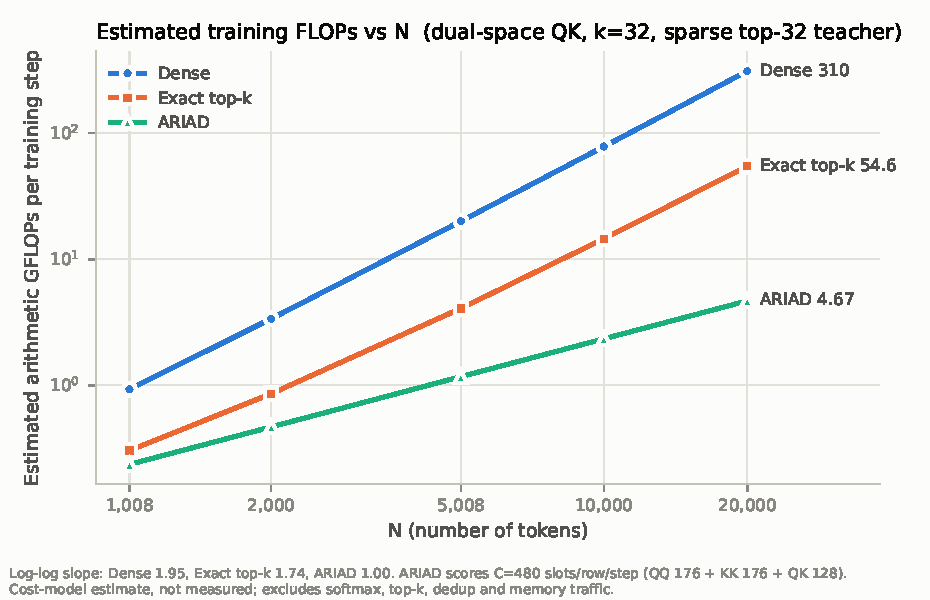
\includegraphics[width=\linewidth]{figures/dual_space_cost.pdf}
 \caption{Dual-space estimated arithmetic cost per training step ($10^9$ FLOPs), with attention width 32 and 480 search slots per row across QQ, KK, and QK. The supplied model charges three projections as trainable, although the experimental value projection is frozen; values therefore represent that common accounting convention, not implementation-exact operation counts. Softmax, top-$k$, deduplication, gather/scatter, memory traffic, and evaluation audits are excluded.}
 \label{fig:dual-cost}
\end{figure}

\paragraph{Arithmetic cost.}
Figure~\ref{fig:dual-cost} uses the supplied three-projection cost model,
\begin{align}
F={}&6N d_{\mathrm{in}}(2d_z+d_v)\nonumber\\
 &+6P_{\mathrm{attn}}(d_z+d_v)+2P_{\mathrm{search}}d_z,
\end{align}
with $d_{\mathrm{in}}=128$ and $d_z=d_v=64$. The attention/search counts are $(N^2,0)$ for Dense, $(32N,N^2)$ for Exact, and $(32N,480N)$ for ARIAD. As in the single-space model, multiply-adds count as two FLOPs and differentiable work as three forward computations. This convention overcounts value-related backward work for the frozen-value experiment. Under this convention, costs at $N=20000$ are $310.15$, $54.64$, and $4.67$ GFLOPs for Dense, Exact, and ARIAD, respectively; ARIAD uses approximately $8.5\%$ of Exact's estimate. Its configured search-score count is $480/20000=2.4\%$ of Exact's. Linear modeled arithmetic assumes fixed dimensions and graph budgets and does not establish end-to-end runtime scaling or hardware speedup.

\begin{figure}[t]
 \centering
 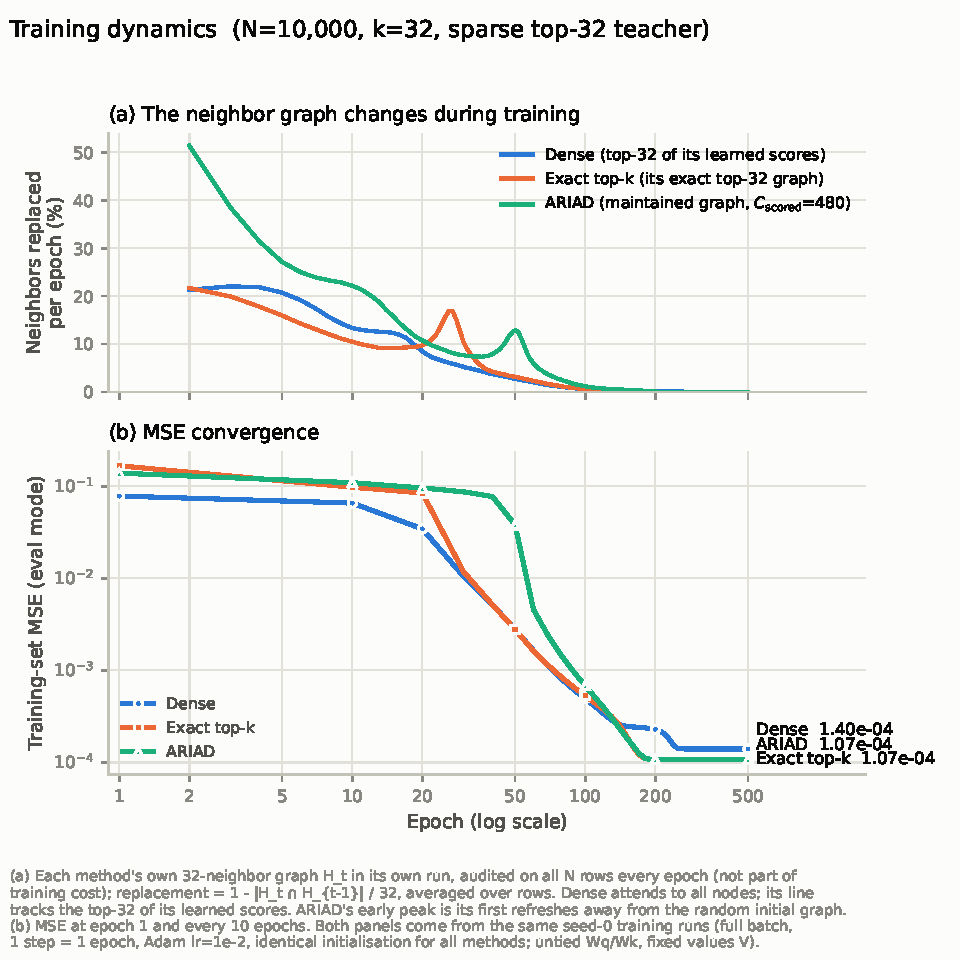
\includegraphics[width=\linewidth]{figures/dual_space_dynamics.pdf}
 \caption{Dual-space training dynamics at $N=10000$, seed 0. (a) Percentage of neighbors replaced between consecutive epochs, averaged over all query rows. Each method uses its own trajectory: Dense's diagnostic top-32, Exact's exact top-32, or ARIAD's maintained QK graph. (b) Post-update training-node MSE at epoch 1 and every ten epochs. The full-row turnover audits are distinct from the 1000-row current-graph recall estimates and are excluded from training costs. One epoch is one optimization step; neither panel measures wall-clock time.}
 \label{fig:dual-dynamics}
\end{figure}

\paragraph{Training dynamics.}
Figure~\ref{fig:dual-dynamics} presents the representative seed-0 runs at $N=10000$. ARIAD replaces $51.4\%$ of its QK neighbors at epoch 2, compared with approximately $21\%$ for the other methods, as it moves away from its random initial graph. In this run, ARIAD's MSE reduction initially lags behind Exact, then approaches its final output quality: at step 500, both have MSE $1.07\times10^{-4}$, versus $1.40\times10^{-4}$ for Dense. Turnover decreases toward zero for all methods. Because these curves describe different learned graphs, similar turnover does not imply agreement of neighbor sets; the sampled current-graph recall separately quantifies retrieval accuracy. This single-seed trajectory does not establish a general convergence-rate ranking.

These results support online graph maintenance with independent query and key projections in this controlled fixed-value setting. The stronger agreement with Exact than in the single-space sweep cannot be attributed to the dual-space construction alone: the teacher, data, value parameterization, and search budget all change. A dual-space budget sweep and experiments with learned values remain outside this evaluation.
